\appendix

\chapter{Supplement to Production Study I} 
\label{Appendix A}

\section{Reading material}

\textbf{Story 1}: Lehrer `teacher' – Geige `violin'\\

NEW-NEW:

\begin{enumerate}
\item Peter ist richtig müde von der Arbeit.
\item Er hat den ganzen Tag im Fundbüro für Besucher Gegenstände herausgesucht.
\item Unter anderem hat er einem Lehrer eine Geige gezeigt.
\item Jetzt ruht er sich vor dem Fernseher aus.
\end{enumerate}

NEW-ACCESSIBLE:

\begin{enumerate}
\item Peter ist richtig müde von der Arbeit.
\item Er hat heute dutzende Besucher durch die kleine Instrumentensammlung im Stadtmuseum geführt.
\item Unter anderem hat er einem Lehrer die Geige gezeigt.
\item Jetzt ruht er sich vor dem Fernseher aus.
\end{enumerate}

ACCESSIBLE-NEW:

\begin{enumerate}
\item Peter ist richtig müde von der Arbeit.
\item Er hat heute eine Schulklasse durch das historische Stadtmuseum geführt.
\item Unter anderem hat er dem Lehrer eine Geige gezeigt.
\item Jetzt ruht er sich vor dem Fernseher aus.
\end{enumerate}

ACCESSIBLE-ACCESSIBLE:

\begin{enumerate}
\item Peter ist richtig müde von der Arbeit.
\item Er hat heute eine Schulklasse durch die kleine Instrumentensammlung im Stadtmuseum geführt.
\item Unter anderem hat er dem Lehrer die Geige gezeigt.
\item Jetzt ruht er sich vor dem Fernseher aus.
\end{enumerate}

\textbf{Story 2}: Nonne `nun' – Mühle `mill'\\

NEW-NEW:

\begin{enumerate}
\item Tom ist richtig müde von der Arbeit.
\item Er hat den ganzen Tag Touristen durch das Stadtmuseum geführt.
\item Unter anderem hat er einer Nonne eine Mühle gezeigt.
\item Jetzt setzt er sich zum Entspannen in seinen Lieblingssessel.
\end{enumerate}

NEW-ACCESSIBLE:

\begin{enumerate}
\item Tom ist richtig müde von der Arbeit.
\item Er hat heute dutzende Besucher durch das Brotmuseum geführt.
\item Unter anderem hat er einer Nonne die Mühle gezeigt.
\item Jetzt setzt er sich zum Entspannen in seinen Lieblingssessel.
\end{enumerate}

ACCESSIBLE-NEW:

\begin{enumerate}
\item Tom ist richtig müde von der Arbeit.
\item Er hat heute eine Gruppe aus der Klosterschule durch das Stadtmuseum geführt.
\item Unter anderem hat er der Nonne eine Mühle gezeigt.
\item Jetzt setzt er sich zum Entspannen in seinen Lieblingssessel.
\end{enumerate}

ACCESSIBLE-ACCESSIBLE:

\begin{enumerate}
\item Tom ist richtig müde von der Arbeit.
\item Er hat heute eine Gruppe aus der Klosterschule durch das Brotmuseum geführt.
\item Unter anderem hat er der Nonne die Mühle gezeigt.
\item Jetzt setzt er sich zum Entspannen in seinen Lieblingssessel.
\end{enumerate}

\textbf{Story 3}: Anwalt `lawyer' – Säge `saw'\\

NEW-NEW:

\begin{enumerate}
\item Jana ist richtig müde von der Arbeit.
\item Sie hat den ganzen Tag im Fundbüro für Kunden Gegenstände herausgesucht.
\item Unter anderem hat sie einem Anwalt eine Säge gezeigt.
\item Jetzt setzt sie sich mit einem Buch auf ihr Sofa.
\end{enumerate}

NEW-ACCESSIBLE:

\begin{enumerate}
\item Jana ist richtig müde von der Arbeit.
\item Sie hat heute dutzende Besucher durch die kleine historische Werkzeugsammlung im Museum geführt.
\item Unter anderem hat sie einem Anwalt die Säge gezeigt.
\item Jetzt setzt sie sich mit einem Buch auf ihr Sofa.
\end{enumerate}

ACCESSIBLE-NEW:

\begin{enumerate}
\item Jana ist richtig müde von der Arbeit.
\item Sie war heute bei einem Gerichtsprozess für die Beweisstücke zuständig.
\item Unter anderem hat sie dem Anwalt eine Säge gezeigt.
\item Jetzt setzt sie sich mit einem Buch auf ihr Sofa.
\end{enumerate}

ACCESSIBLE-ACCESSIBLE:

\begin{enumerate}
\item Jana ist richtig müde von der Arbeit.
\item Sie war heute bei einem Gerichtsprozess für die Beweisstücke zum Mord im Baumarkt zuständig.
\item Unter anderem hat sie dem Anwalt die Säge gezeigt.
\item Jetzt setzt sie sich mit einem Buch auf ihr Sofa.
\end{enumerate}
 
\textbf{Story 4}: Bauer `farmer' – Birne `pear'\\

NEW-NEW:

\begin{enumerate}
\item Nach zwei regnerischen Wochen schien endlich wieder die Sonne.
\item Maria hat sich ihre Schuhe angezogen und ist spazieren gegangen. 
\item Unterwegs hat sie einem Bauern eine Birne geschenkt.
\item Jetzt ist sie wieder zu Hause und kocht sich einen Tee.
\end{enumerate}

NEW-ACCESSIBLE:

\begin{enumerate}
\item Nach zwei regnerischen Wochen schien endlich wieder die Sonne.
\item Nachdem Maria ein paar Früchte eingesteckt hatte, ist sie spazieren gegangen.
\item Unterwegs hat sie einem Bauern die Birne geschenkt.
\item Jetzt ist sie wieder zu Hause und kocht sich einen Tee.
\end{enumerate}

ACCESSIBLE-NEW:

\begin{enumerate}
\item Nach zwei regnerischen Wochen schien endlich wieder die Sonne.
\item Maria hat sich ihre Schuhe angezogen und ist zwischen den Feldern des benachbarten Gutshofs spazieren gegangen. 
\item Unterwegs hat sie dem Bauern eine Birne geschenkt.
\item Jetzt ist sie wieder zu Hause und kocht sich einen Tee.
\end{enumerate}

ACCESSIBLE-ACCESSIBLE

\begin{enumerate}
\item Nach zwei regnerischen Wochen schien endlich wieder die Sonne.
\item Nachdem Maria ein paar Früchte eingesteckt hatte, ist sie zwischen den Feldern des benachbarten Gutshofs spazieren gegangen.
\item Unterwegs hat sie dem Bauern die Birne geschenkt.
\item Jetzt ist sie wieder zu Hause und kocht sich einen Tee.
\end{enumerate}

\textbf{Story 5}: Maler `painter' – Waage `scale'\\

NEW-NEW:

\begin{enumerate}
\item Anna hatte einen erfolgreichen Tag.
\item Sie hat die Kunden auf dem Flohmarkt für viele ihrer Waren begeistern können.
\item Unter anderem hat sie einem Maler eine Waage verkauft.
\item Jetzt ist sie zu Hause und entspannt sich bei schöner Musik.
\end{enumerate}

NEW-ACCESSIBLE:

\begin{enumerate}
\item Anna hatte einen erfolgreichen Tag im Geschäft.
\item Sie hat die Kunden für die Restbestände bei den Küchengeräten begeistern können. 
\item Unter anderem hat sie einem Maler die Waage verkauft.
\item Jetzt ist sie zu Hause und entspannt sich bei schöner Musik.
\end{enumerate}

ACCESSIBLE-NEW:

\begin{enumerate}
\item Anna hatte einen erfolgreichen Tag.
\item Am Mittag sind einige Handwerker von der Baustelle nebenan in ihr Geschäft gekommen.
\item Unter anderem hat sie dem Maler eine Waage verkauft.
\item Jetzt ist sie zu Hause und entspannt sich bei schöner Musik.
\end{enumerate}

ACCESSIBLE-ACCESSIBLE:

\begin{enumerate}
\item Anna hatte einen erfolgreichen Tag.
\item Am Mittag sind einige Handwerker von der Baustelle nebenan in ihr Geschäft gekommen, um sich die Restbestände bei den Küchengeräten anzusehen.
\item Unter anderem hat sie dem Maler die Waage verkauft.
\item Jetzt ist sie zu Hause und entspannt sich bei schöner Musik.
\end{enumerate}

\textbf{Story 6}: Kellner `server' – Vase `vase'\\

NEW-NEW:

\begin{enumerate}
\item Claudia hatte einen erfolgreichen Tag.
\item Sie hat die Kunden auf dem Flohmarkt für viele ihrer Waren begeistern können.
\item Unter anderem hat sie einem Kellner eine Vase verkauft.
\item Jetzt geht sie nach Hause und legt sich sofort hin.
\end{enumerate}

NEW-ACCESSIBLE:

\begin{enumerate}
\item Claudia hatte einen erfolgreichen Tag.
\item Sie hat die Kunden in ihrem Blumenladen für die restlichen Keramikartikel begeistern können. 
\item Unter anderem hat sie einem Kellner die Vase verkauft.
\item Jetzt geht sie nach Hause und legt sich sofort hin.
\end{enumerate}

ACCESSIBLE-NEW:

\begin{enumerate}
\item Claudia hatte einen erfolgreichen Tag im Geschäft.
\item Sie hat einige Kollegen vom Restaurant nebenan für viele ihrer Waren begeistern können.
\item Unter anderem hat sie dem Kellner eine Vase verkauft.
\item Jetzt geht sie nach Hause und legt sich sofort hin.
\end{enumerate}

ACCESSIBLE-ACCESSIBLE:

\begin{enumerate}
\item Claudia hatte einen erfolgreichen Tag.
\item Sie hat einige Kollegen vom Restaurant nebenan für die restlichen Keramikartikel in ihrem Blumenladen begeistern können.
\item Unter anderem hat sie dem Kellner die Vase verkauft.
\item Jetzt geht sie nach Hause und legt sich sofort hin.
\end{enumerate}
 
\textbf{Story 7}: Oma `grandma' – Mantel `coat'\\

NEW-NEW:

\begin{enumerate}
\item Rudi hatte einen erfolgreichen Tag.
\item An seinem Stand auf dem Flohmarkt sind viele Leute vorbeigekommen.
\item Unter anderem hat er einer Oma einen Mantel verkauft.
\item Jetzt entspannt er sich in der Badewanne.
\end{enumerate}

NEW-ACCESSIBLE:

\begin{enumerate}
\item Rudi hatte einen erfolgreichen Tag.
\item Viele Kunden haben sich in seiner Boutique für die Einzelstücke der Herbst-Kollektion interessiert.
\item Unter anderem hat er einer Oma den Mantel verkauft.
\item Jetzt entspannt er sich in der Badewanne.
\end{enumerate}

ACCESSIBLE-NEW:

\begin{enumerate}
\item Rudi hatte einen erfolgreichen Tag.
\item Unter den Kunden an seinem Stand auf dem Flohmarkt war auch eine Großfamilie.
\item Unter anderem hat er der Oma einen Mantel verkauft.
\item Jetzt entspannt er sich in der Badewanne.
\end{enumerate}

ACCESSIBLE-ACCESSIBLE:

\begin{enumerate}
\item Rudi hatte einen erfolgreichen Tag.
\item Unter den Kunden in seiner Boutique war auch eine Großfamilie, die sich für die Einzelstücke der Herbst-Kollektion interessiert hat.
\item Unter anderem hat er der Oma den Mantel verkauft.
\item Jetzt entspannt er sich in der Badewanne.
\end{enumerate}

\textbf{Story 8}: Sänger `singer' – Kanne `can'\\

NEW-NEW:

\begin{enumerate}
\item Sandra hatte einen erfolgreichen Tag.
\item An ihrem Stand auf dem Flohmarkt sind viele Leute vorbeigekommen.
\item Unter anderem hat sie einem Sänger eine Kanne verkauft.
\item Jetzt kocht sie sich Nudeln zum Abendessen.
\end{enumerate}

NEW-ACCESSIBLE:

\begin{enumerate}
\item Sandra hatte einen erfolgreichen Tag in ihrem Teeladen.
\item Einige Kunden haben sich für die Einzelstücke der Porzellankollektion aus dem Vorjahr interessiert.
\item Unter anderem hat sie einem Sänger die Kanne verkauft.
\item Jetzt kocht sie sich Nudeln zum Abendessen.
\end{enumerate}

ACCESSIBLE-NEW:

\begin{enumerate}
\item Sandra hatte einen erfolgreichen Tag auf dem Flohmarkt.
\item Es war viel los und wie immer gab es auch ein Live-Konzert. 
\item Unter anderem hat sie dem Sänger eine Kanne verkauft.
\item Jetzt kocht sie sich Nudeln zum Abendessen.
\end{enumerate}

ACCESSIBLE-ACCESSIBLE:

\begin{enumerate}
\item Sandra hatte einen erfolgreichen Tag auf dem Flohmarkt. 
\item Wie immer gab es auch ein Live-Konzert und einige Leute haben sich für das alte Teeservice ihrer Oma interessiert.
\item Unter anderem hat sie dem Sänger die Kanne verkauft.
\item Jetzt kocht sie sich Nudeln zum Abendessen.
\end{enumerate}

\textbf{Practice stories}\\

Rabbi `rabbi' - Angel `fishing rod'\\

NEW-NEW:

\begin{enumerate}
\item Georg ist müde von der Arbeit.
\item Er hat den ganzen Tag im Fundbüro für Besucher Gegenstände herausgesucht.
\item Zum Schluss hat er einem Rabbi eine Angel gezeigt.
\item Jetzt geht er in seine Lieblingskneipe.
\end{enumerate}

Mutter `mother' - Lampe `lamp'\\

NEW-NEW:

\begin{enumerate}
\item Heute Morgen waren viele Kunden im Geschäft.
\item David war die ganze Zeit damit beschäftigt, Fragen zu beantworten.
\item Dann hat er einer Mutter eine Lampe verkauft.
\item Jetzt macht er Mittagspause.
\end{enumerate}

\newpage

\section{Accent types by speaker}

\begin{figure}
		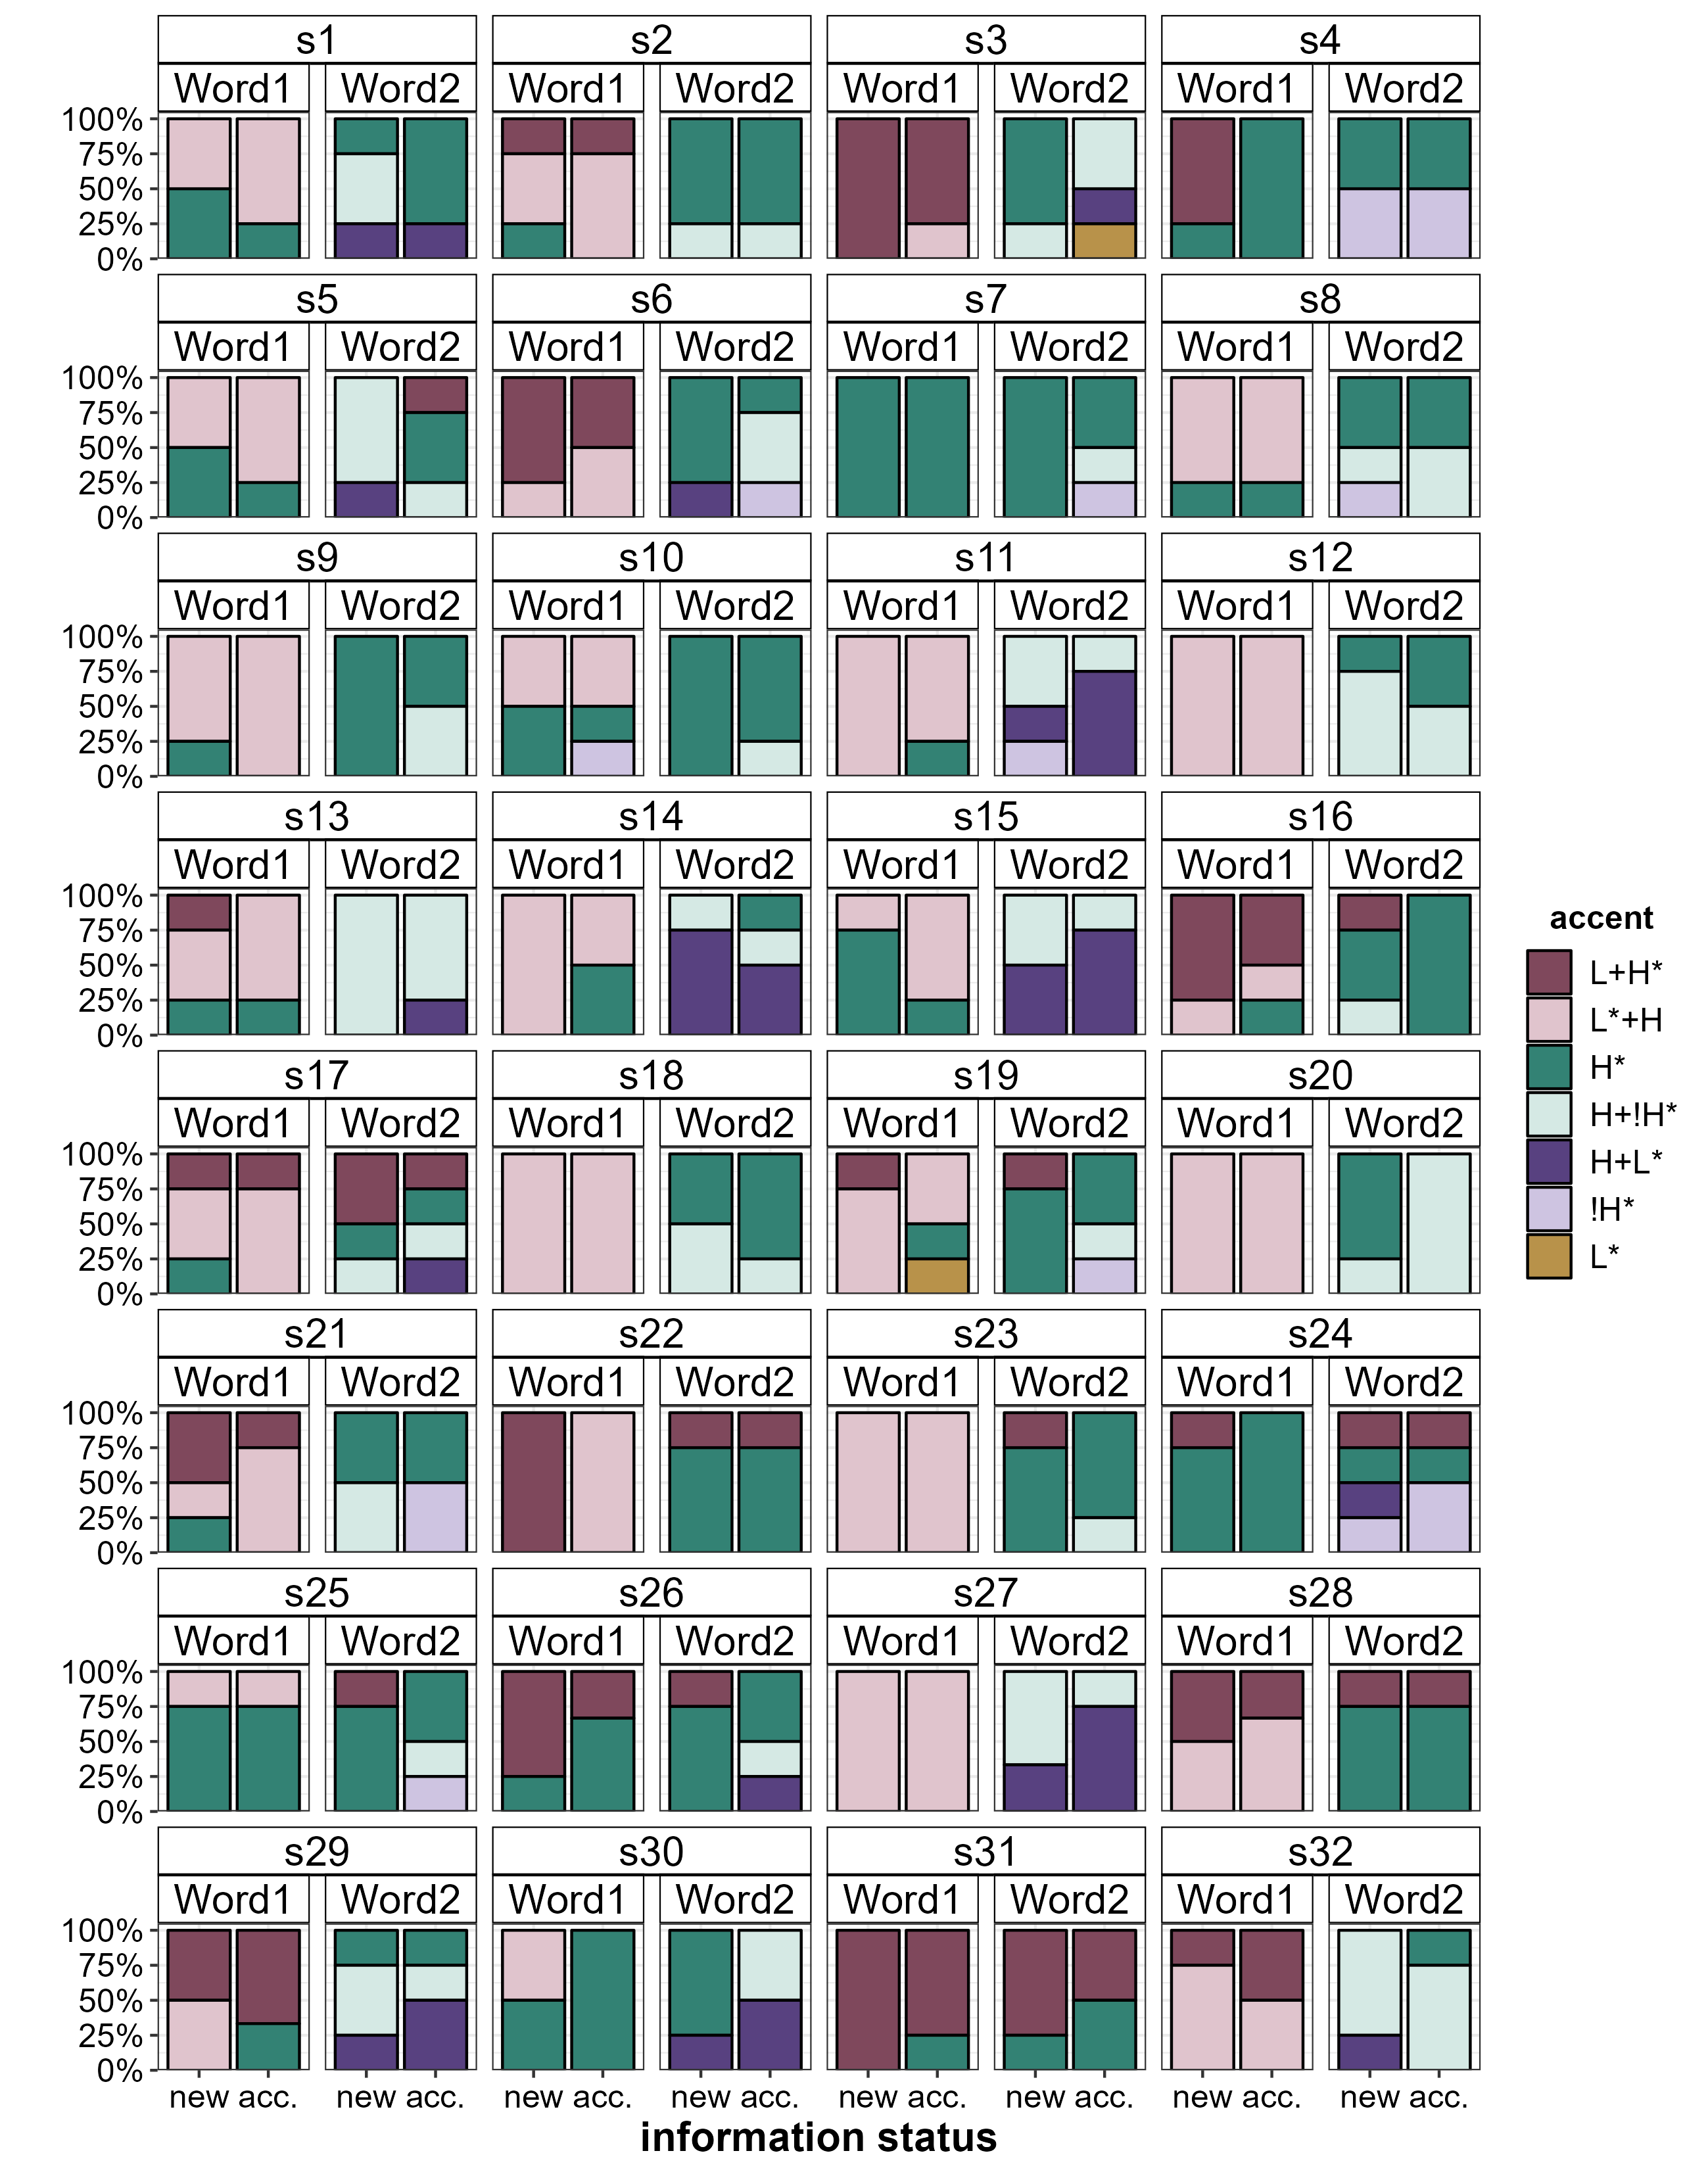
\includegraphics[scale = 0.55]{s1_accent_type_byspeaker_all}
	\caption{Barplots of the distributions of accent type by position and information status for each speaker.}	\label{fig:s1_accent_type_byspeaker_all}
\end{figure}
